\documentclass[../main.tex]{subfiles}

\graphicspath{{../images/}}

\begin{document}
\pagestyle{fancy}
\lhead{Lecture 7: 9/17/24}
\chead{Chapter 3}
\rhead{PHYS 421}

\section{Potentials}
\barh \vspace{1em}

\subsection{Laplace's Equation}

\subsubsection{Intro}
In principle, electrostatis is
\begin{align*}
    \vb E (\vb r) = \ke \int \frac{\vu\scriptr}{\scriptr^2} \rho(\vb r') \dd\tau', \quad \vb \scriptr = \vb r - \vb r'
\end{align*}
And simplifying with potential
\begin{align*}
    V(\vb r) = \ke \int \frac{\rho(\vb r')}{\scriptr} \dd \tau'
\end{align*}
So we often use Poisson's equation e.g.
\begin{align*}
    \laplacian V = -\frac{\rho}{\epsilon_0}
\end{align*}
Even better, Laplace's equation
\begin{align*}
    \boxed{\laplacian V = 0}
\end{align*}
or in Cartesian
\begin{align*}
    \laplacian V = \pdv[2]{V}{x} + \pdv[2]{V}{y} + \pdv[2]{V}{z} = 0
\end{align*}

\subsubsection{Start in 1D}
\begin{align*}
    \pdv[2]{V}{x} = 0 \implies V = mx + b
\end{align*}
where we have two undetermined constants $m$ \& $b$.
We can determine these constants by \textit{boundary conditions}.
\begin{itemize}
    \item e.g. $V(1) = 4 \quad V(5) = 0$; we get a line $V = -\frac{4}{5}x + 4$
\end{itemize}

\paragraph{Two features:}
\begin{enumerate}
    \item $V(x)$ is average of $V(x + a)$ and $V(x - a)$
    \begin{align*}
        V(x) = \frac{1}{2} \qt[V(x + a) + V(x - a)]
    \end{align*}
    \item \textbf{NO} local minima or maxima (no curvature!)
\end{enumerate}

\newpage
\subsubsection{On to 2D}
\begin{align*}
    \pdv[2]{V}{x} + \pdv[2]{V}{y} = 0 \qqtext{no general solution}
\end{align*}
and no requirement on the \# of constants.
But we can note common properties e.g. soap film on a wireframe assumes the same shape.
\begin{figure*}[ht]
    \centering
    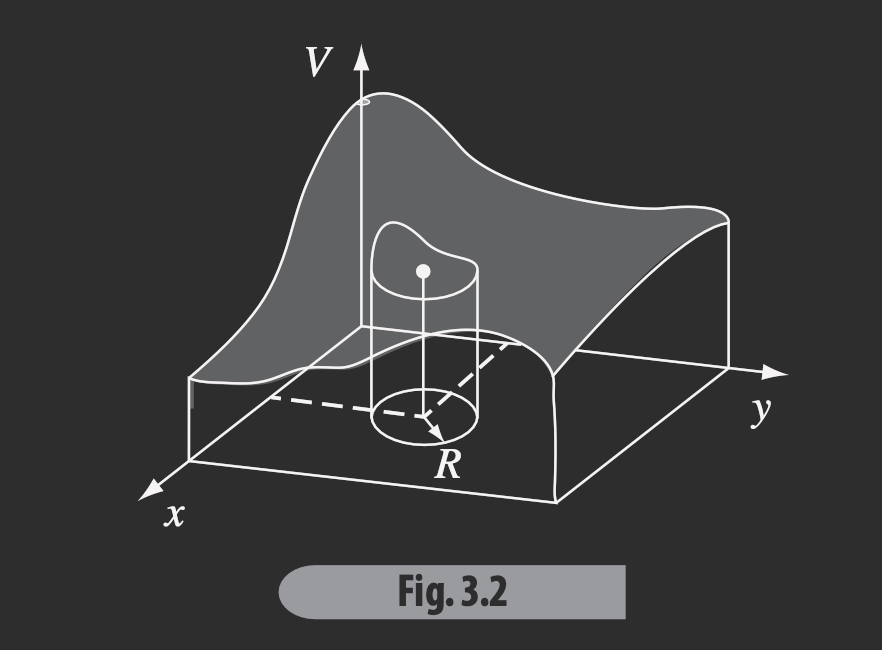
\includegraphics[width=0.3\linewidth]{fig3_2.png}
    \caption{}
    \label{fig:lecture3_2}
\end{figure*}
The solutions are called \textit{harmonic functions}:
\begin{enumerate}
    \item value $V(x,y)$ is average of nearby values; more precisely, for a circle of radius $R$ (Fig. \ref{fig:lecture3_2})
    \begin{align*}
        V(x,y) = \frac{1}{2\pi R} \oint V \dd\ell
    \end{align*}
    where $2\pi R$ is the circumference of the circle.
    \item \textbf{NO} local minima or maxima
\end{enumerate}

\subsubsection{In 3D}
\begin{align*}
    \laplacian V = 0
\end{align*}
Holds same properties as 2D:
\begin{enumerate}
    \item Average over spherical surface of radius $R$ centered at $\vb r$:
    \begin{align*}
        V(\vb r) = \frac{1}{4\pi R^2} \oint_S V \dd a
    \end{align*}
    where $4\pi R^2$ is the surface area of the sphere.
\end{enumerate}

\paragraph{Example:} Point charge outside sphere; The potential at $\dd a$
\begin{align*}
    V = \ke \frac{q}{\scriptr} 
\end{align*}
and from law of cosines 
\begin{align*}
    \scriptr^2 = z^2 + R^2 - 2rR\cos\theta
\end{align*}
so the average potential is
\begin{align*}
    V_\text{avg} &= \frac{q}{4\pi R^2} \ke \int \frac{R^2 \sin\theta \dd\theta \dd\phi}{\sqrt{z^2 + R^2 - 2zR\cos\theta}} \\
    &= \frac{q}{2zR} \ke \qt[z^2 + R^2 - 2zR\cos\theta]^{1/2} \eval_0^\pi \\
    &= \frac{q}{2zR} \ke \qt[(z + R) - (z - R)] \\
    &= \ke \frac{q}{z}
\end{align*}
which is just the potential of a point charge $q$ in the center of the sphere.

\paragraph{Question:} Is it possible to stably trap a charged particle using electrostatic forces alone? 

\paragraph{Answer} Earnshaw's theorem: A charged particle cannot be held in stable equilibrium by electrostatic forces alone.

\subsubsection{Boundary Conditions \& Uniqueness Theorem}

Laplace's eq requires boundary conditions (b.c.c)

\paragraph{1st uniqueness theorem:}

``Solutions to L's eq in volume $V$ is uniquely determined if potential is specied in surface $S$ bounding $V$.''

How is the solution unique?

Have solution in $V_1$ s.l.
\begin{align*}
    \laplacian V_1 = 0 \qqtext{also} \laplacian V_2 = 0
\end{align*}
Then
\begin{align*}
    V_3 \equiv \Delta V = V_1 - V_2
\end{align*}
which means
\begin{align*}
    \laplacian V_3 = \laplacian V_1 - \laplacian V_2 = 0 - 0 = 0
\end{align*}
thus
\begin{align*}
    \implies \laplacian V_1 &= \laplacian V_2 \\
    V_1 &= V_2
\end{align*}
We should emphasize that $V_1$ defined on the boundary $S$ is also the same b.c.s as $V_2$ while $V_3$ on the boundary equals zero.
That is $V_3$ is zero everywhere in space.

\subsubsection{2nd uniqueness theorem (conductors):}

``In a volume $V$ surrounded by conductors, and containing a specifed charge density $\rho$,
then the $\vb E$ field is uniquely determined if the total charge on each conductor is given.''

``This proof was not easy'' - Griffiths

\paragraph{Example:} Connecting two pairs of opposite charges with a conductor;
what is the final charge config and E-field?

\paragraph{Answer:} $\vb E = 0$ everywhere. The total charge of each conductor is zero.

\subsubsection{Boundary conditions pt. II}

(Griffiths 2.3.5 pg 85) Given a sheet of charge $\sigma = Q/ A$ and using the Gaussian pillbox method 
\begin{align*}
    \oint \vb E \cdot \dd\vb a &= \frac{q_\text{enc}}{\epsilon_0} \\
    E_a A - E_b A &= \sigma \frac{A}{\epsilon_0} \\
    E_a - E_b &= \frac{\sigma}{\epsilon_0}
\end{align*}

For the same surface we know that
\begin{align*}
    \curl \vb E = \oint \vb E \cdot \dd\ell = 0
\end{align*}
So going around the loop we have
\begin{align*}
    E_a \ell - E_b \ell &= 0 \\
    E_a &= E_b
\end{align*}

\newpage
\subsection{Method of Images}
\lhead{Lecture 8: 9/19/24}

$\laplacian V = -\rho/\epsilon_0$ \textit{is} electrostatics. AND when we have $\laplacian V = 0$, Uniqueness theorems tell us there is a solution,
but doesn't tell us how to find it\dots thus we have a set of ``easily'' solvable problems.

\subsubsection{Classic image problem:}

``Ground'' is infinite conducting plane $V = 0$ at $z = 0$. For a charge $q$ at $z = d$ what is the potential in $z > 0$?
We know that the point charge will induce a charge on the plane which will effect the electic potential in the region $z > 0$.
% fig3_10
\begin{figure*}[ht]
    \centering
    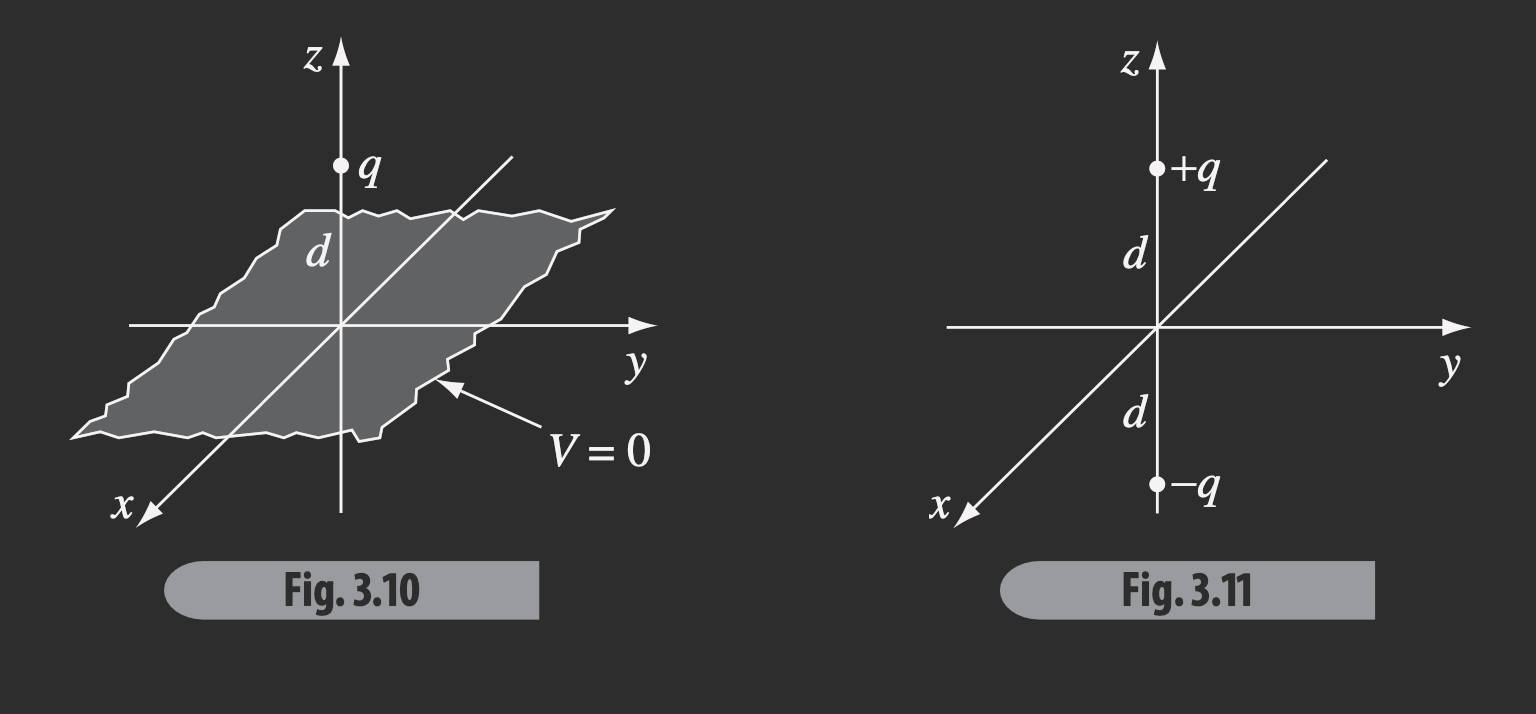
\includegraphics[width=0.5\linewidth]{fig3_10.png}
    \caption{}
    \label{fig:lecture3_10}
\end{figure*}

\paragraph{GOAL: } solve $\laplacian V = -\rho/\epsilon_0$ for $z \geq 0$ 
with $+q$ at $(0,0,d)$ subject to boundary conditions (b.c.s)
\begin{enumerate}
    \item $V(z=0) = 0$ 
    \item $V \to 0$ for far away
\end{enumerate}
The next step is to replace the conducting plane with an equivalent charge $-q$ at $z = -d$.

NOTE: We only care about $z \geq 0$ and ignore $z < 0$ region; furthermore, the potential below the plane should be zero as the boundary of the plane sort of ``wraps'' around the charge

Thus the solution is a superposition of charges
\begin{align*}
    V = \ke \qt[\frac{q}{\sqrt{x^2 + y^2 + (z-d)^2}} - \frac{q}{\sqrt{x^2 + y^2 + (z+d)^2}}]
\end{align*}
we can see that in the replacement problem, the region below the grounded plane is nonzero which is different from the real problem which is why we ignore it!

\subsubsection{Induced surface charge} 

What is $\sigma$? Recall on the sheet $\sigma$ we have a field
\begin{align*}
    \vb E_\textrm{ab} - \vb E_\textrm{be} = \frac{\sigma}{\epsilon_0} \vu n
\end{align*}
where the $\vu n$ tells us that we are dealing with the perpendicular planes; thus the same eq
\begin{align*}
    \grad V_\text{ab} - \grad V_\text{be} = -\frac{\sigma}{\epsilon_0} \vu n \implies \vb E = -\grad V
\end{align*}
We can infer that
\begin{align*}
    \pdv{V_a}{n} - \cancel{\pdv{V_b}{n}} = -\frac{\sigma}{\epsilon_0}
\end{align*}
since anything below the plane is zero from the previous example. We know have
\begin{align*}
    \pdv{V_a}{z} \eval_{z\to 0} &= \ke \qt[-\frac{q(z-d)}{(x^2 + y^2 + (z-d)^2)^{3/2}} + \frac{q(z+d)}{(x^2 + y^2 + (z+d)^2)^{3/2}}] \eval_{z\to 0}
\end{align*}
So
\begin{align*}
    \sigma = -\frac{1}{2\pi} \frac{qd}{(x^2 + y^2 + d^2)^{3/2}}
\end{align*}
We can check that the total induced charge in the plane is infact
\begin{align*}
    Q = \int_0^{2\pi} \int_0^\infty \sigma  r\dd r \dd\phi = - q
\end{align*}
where $r^2 = x^2 + y^2$.

This charge comes from the reservoir of charge given by ground.

\begin{figure*}[ht]
    \centering
    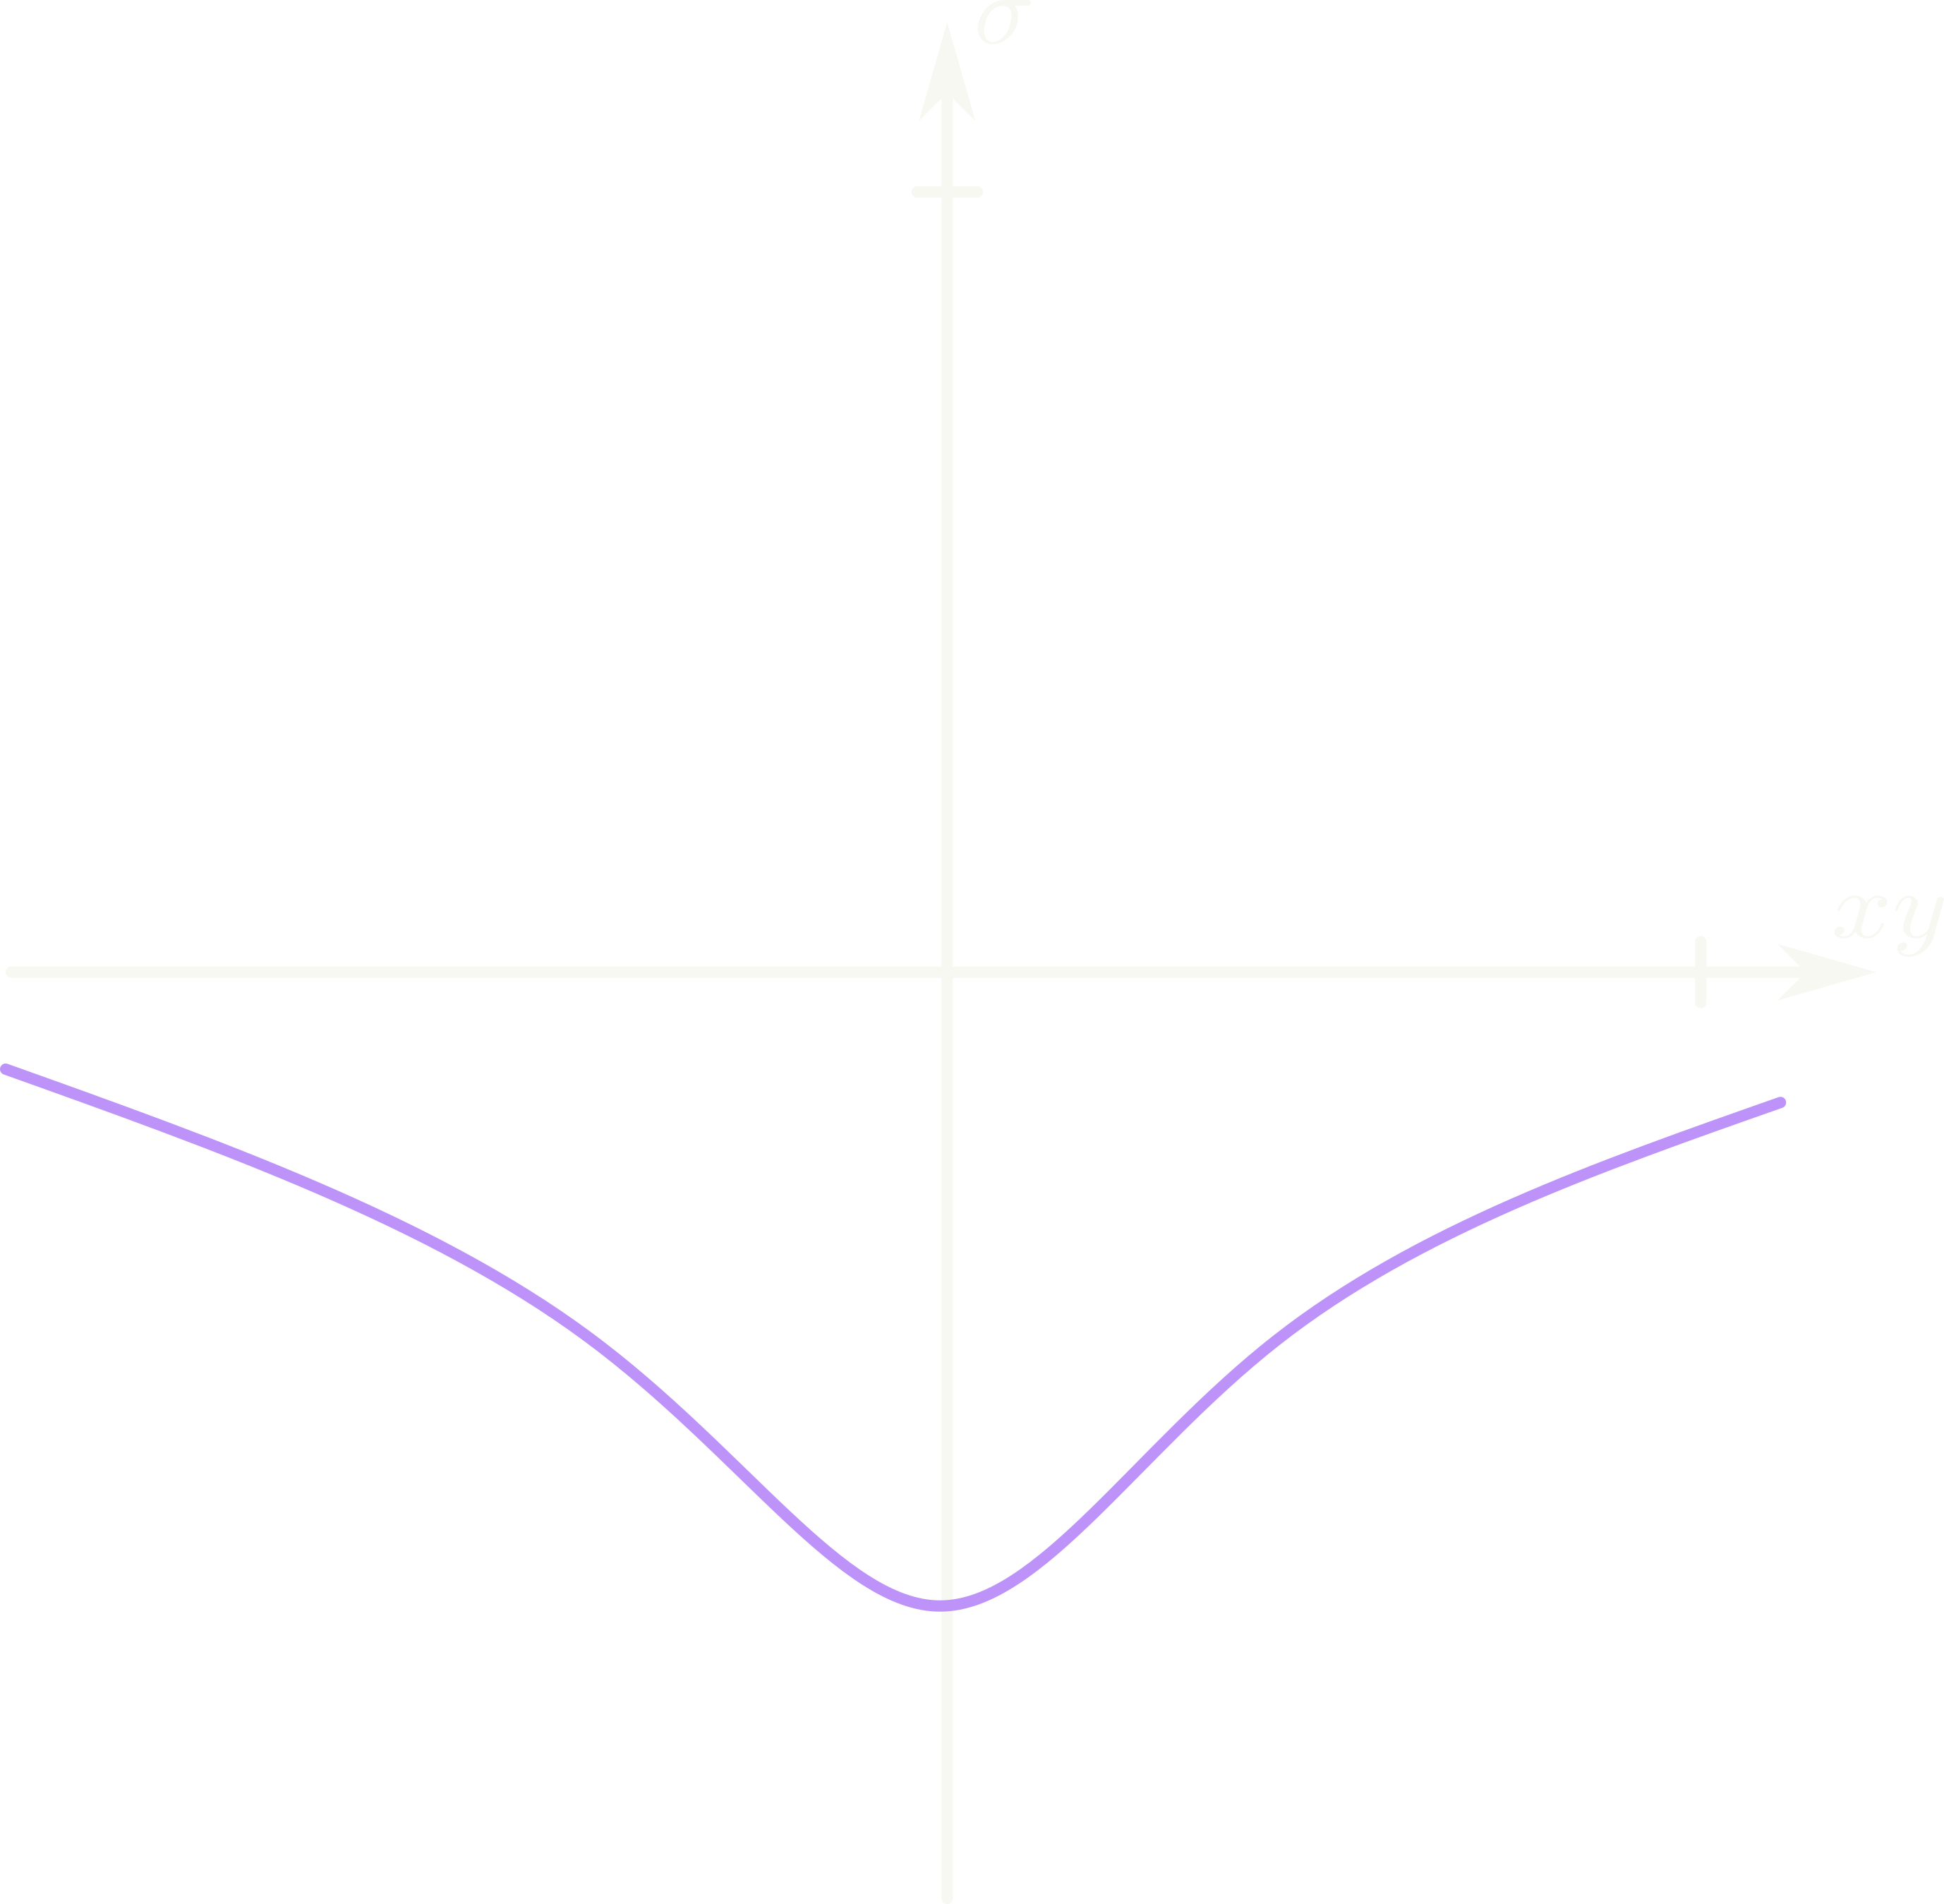
\includegraphics[width=0.3\linewidth]{fig3_11.png}
    \caption{Just a cool graph of $xy$ vs $\sigma$}
    \label{fig:lecture3_11}
\end{figure*}

\subsubsection{Force and energy}

Calcuating the force of attraction because of the negative induced charge:
\begin{align*}
    F = qE = \ke \frac{q^2}{(2d)^2} (-\vu z)
\end{align*}
Naively, we calculate the energy/work done as
\begin{align*}
    W = -\ke \frac{q^2}{2d} \quad (=q \Delta V)
\end{align*}
but we only have a single charge and the total work is half of this value
\begin{align*}
    W = -\ke \frac{q^2}{4d}
\end{align*}
This is because the ideal conductor requires no work to build up a charge distribution $\sigma$.

\newpage
\lhead{Lecture 9: 9/24/24}
Thus we have two ODEs
\subsection{Seperation of Variables}

\subsubsection{In Cartesian}
\begin{figure*}[ht]
    \centering
    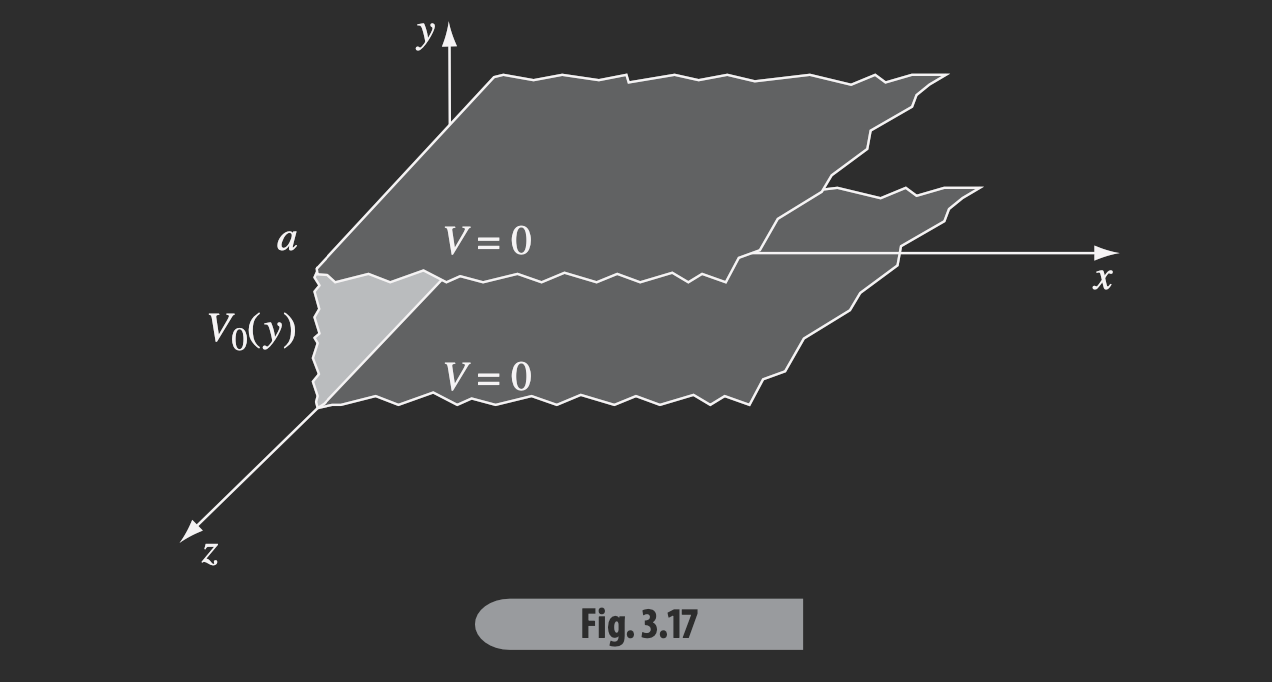
\includegraphics[width=0.5\linewidth]{fig3_17.png}
    \caption{3 planes where top and bottom are grounded and the middle is at $V_0(y)$}
    \label{fig:lecture3_17}
\end{figure*}

Find potential $V$ in $x > 0$, $0< y < a$, $-\infty < z < \infty$:

This is a 2D problem $V\to V(x,y)$

No change in $V \to \laplacian V = 0 = \pdv[2]{V}{x} + \pdv[2]{V}{y}$. 

From b.c.s
\begin{enumerate}
    \item [(i)] $V(y=0) = 0$
    \item [(ii)] $V(y=a) = 0$
    \item [(iii)] $V(x=0) = V_0(y)$
    \item [(iv)] $V(x\to\infty) = 0$
\end{enumerate}

PROPOSE: $V(x,y) = X(x)Y(y)$
\begin{align*}
    \laplacian V &= Y\pdv[2]{X}{x} + X\pdv[2]{Y}{y} = 0 \\
    \frac{\laplacian V}{V} &= \frac{1}{X} \pdv[2]{X}{x} + \frac{1}{Y} \pdv[2]{Y}{y} = 0
\end{align*}
thus we have two independent functions
\begin{align*}
    f(x) + g(y) = 0
\end{align*}
which is \textit{only} possible if both $f$ and $g$ are constants
\begin{align*}
    C_1 + C_2 = 0 \implies C_1 = -C_2 \qor C_1 = C_2 = 0
\end{align*}
We now claim
\begin{align*}
    \sgn(C_1) = 1, \quad \sgn(C_2) = -1, \qand \abs{C_1} = \abs{C_2} = k^2
\end{align*}

\begin{align*}
    \pdv[2]{X}{x} &= k^2 X \\
    \pdv[2]{Y}{y} &= -k^2 Y
\end{align*}
with general solutions
\begin{align*}
    X(x) &= Ae^{kx} + Be^{-kx}, \quad Y(y) = C \sin(ky) + D \cos(ky)
\end{align*}
so the original potential are the product of the two solutions
\begin{align*}
    V(x,y) &= \qt(Ae^{kx} + Be^{-kx}) (C\cos(ky) + D\sin(ky)) \\
    &= e^{-kx} (C \cos(ky) + D \sin(ky))
\end{align*} 
where condition (iv) requires $A = 0$ and condition (i) requires $D = 0$. 
From condition (ii) we require $\sin(ka) = 0$ thus
\begin{align*}
    k = \frac{n\pi}{a},\quad n = 1,2,3,\dots
\end{align*}
Finally from condition (iii) we start with the rewritten potential
\begin{align*}
    V(x,y) = C e^{-kx} \sin(ky) \qquad k = \frac{n\pi}{a}
\end{align*}
We now have an infinite number of solutions
\begin{align*}
    V_1, V_2, V_3, \dots \qif V=\alpha_1 V_1 + \alpha_2 V_2 + \dots
\end{align*}
where the general solution is 
\begin{align*}
    V(x,y) = \sum_{n=1}^\infty C_n e^{-n\pi x/a} \sin(n\pi y/a)
\end{align*}
Now from (iii) we want $V(0,y) \implies V_0(y)$, so we multiply both sides by $\sin(n\pi y/a)$ and integrate over $y$
\begin{align*}
    \sum_{n=1}^\infty C_n \int_0^a \sin(n\pi y/a) \sin(n'\pi y/a) dy = \int_0^a V_0(y) \sin(n'\pi y/a) dy
\end{align*}
where the left integral is evaluated as
\begin{align*}
    \int_0^a \sin(n\pi y/a) \sin(n'\pi y/a) dy =
    \begin{cases}
        0 & n \neq n' \\
        \frac{a}{2} & n = n'
    \end{cases}
\end{align*}
This gives us the coefficient 
\begin{align*}
    C_n = \frac{2}{a} \int_0^a V_0(y) \sin(n\pi y/a) dy
\end{align*}
We let $V_0(y) = V_0 \neq 0$ so
\begin{align*}
    C_n = \frac{2}{a} V_0 \int_0^a \sin(n\pi y/a) dy = \frac{2V_0}{n\pi} (1 - \cos(n\pi)) 
    = \begin{cases}
        0 & n \text{ even} \\
        \frac{4V_0}{n\pi} & n \text{ odd}
    \end{cases}
\end{align*}
so
\begin{align*}
    \boxed{
        V(x,y) = \frac{4V_0}{\pi} \sum_{\textrm{odd } n} \frac{1}{n} e^{-n\pi x/a} \sin(\frac{n\pi y}{a})
    }
\end{align*}
\begin{figure*}[ht]
    \centering
    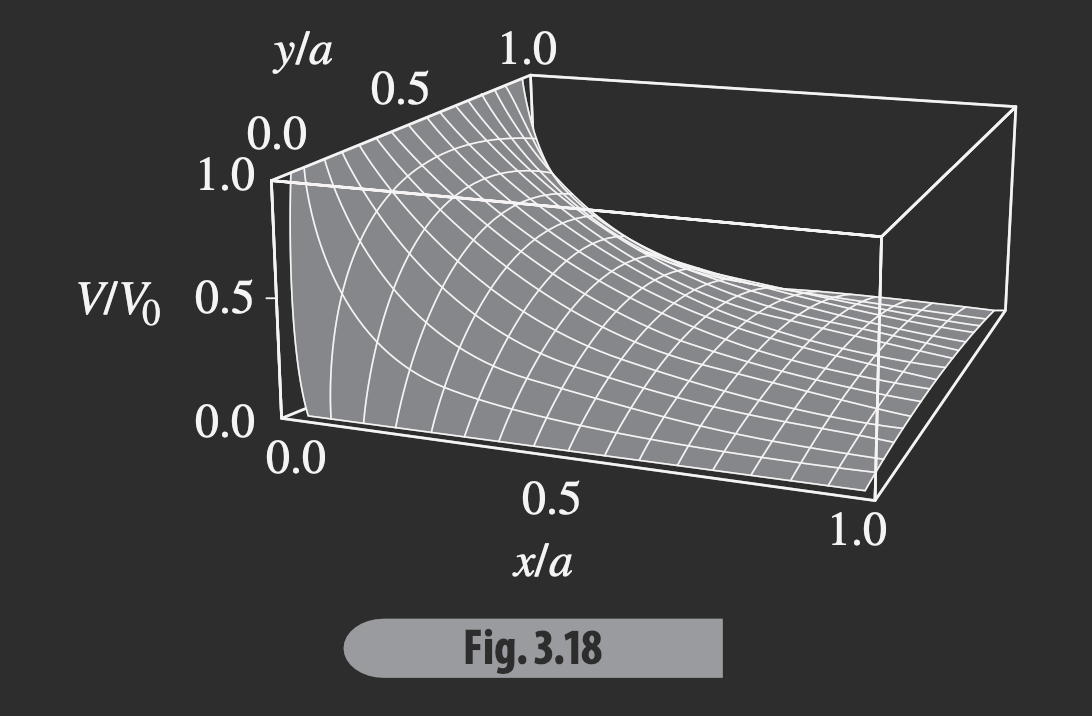
\includegraphics[width=0.5\linewidth]{fig3_18.png}
    \caption{Graph of $V(x,y)$}
    \label{fig:lecture3_18}
\end{figure*}
\newpage
Furthermore, the infinite series can be simplified to
\begin{align*}
    V(x,y) = \frac{2V_0}{\pi} \arctan(\frac{\sin(\frac{\pi y}{a})}{\sinh(\frac{\pi x}{a})})
\end{align*}
We can see this graphed in 3D space in Fig. \ref{fig:lecture3_18}.

\subsubsection{In Spherical}
The laplacian now becomes
\begin{align*}
    \laplacian V = \frac{1}{r^2} \pdv{r}(r^2 \pdv{V}{r}) 
        + \frac{1}{r^2 \sin\theta} \pdv{\theta} (\sin\theta \pdv{V}{\theta})
        + \frac{1}{r^2 \sin^2\theta} \pdv[2]{V}{\phi} = 0
\end{align*}
For the subject matter of undergraduate E\&M, we will assume azimuthal symmetry i.e.
\begin{align*}
    V = V(r, \theta)
\end{align*}
so that $V$ is independent of $\phi$:
\begin{align*}
    \laplacian V = \pdv{r} (r^2 \pdv{V}{r}) + \frac{1}{\sin\theta} \pdv{\theta} (\sin\theta \pdv{V}{\theta}) = 0
\end{align*}
So we look for solutions that are a product two independent functions
\begin{align*}
    V(r, \theta) = R(r) \Theta(\theta)
\end{align*}
thus dividing the laplacian by $V$ we get
\begin{align*}
    \underbrace{
        \frac{1}{R} \pdv{r} (r^2 \pdv{R}{r})
    }_{C_1} 
    + \underbrace{
        \frac{1}{\Theta \sin\theta} \pdv{\theta} (\sin\theta \pdv{\Theta}{\theta}) 
    }_{C_2} = 0
\end{align*}
where $C_1$ and $C_2$ are constants. We now choose
\begin{align*}
    C_1 = \ell (\ell +1), \quad C_2 = -\ell (\ell + 1)
\end{align*}
so that the radial \& polar equation becomes
\begin{align*}
    R(r) = A r^\ell + \frac{B}{r^{\ell + 1}} \\
    \Theta(\theta) = P_\ell(\cos\theta)
\end{align*}
where $P_\ell$ is a Legendre polynomial defined by the Rodrigues formula (there are multiple ways to define this polynomial)
\begin{align*}
    P_\ell(x) &= \frac{1}{2^\ell \ell!} \qt(\dv{x})^\ell (x^2 - 1)^\ell \\
    P_0 &= 1 \\
    P_1 &= x \\
    P_2 &= \frac{1}{2}(3x^2 - 1)\dots
\end{align*}
The most general solution is a linear combination
\begin{align*}
    V_{\text{gen}}(r, \theta) = \sum_{\ell = 0}^\infty \qt(A_\ell r^\ell + \frac{B_\ell}{r^{\ell + 1}}) P_\ell(\cos\theta)
\end{align*}

\paragraph{Example} Uncharged conducting sphere sitting in a background E-field $\vb E = E_0 \vu z$, so far away, the field points directly up.
The induced charge on the sphere has positive charges at the top and negative charges at the bottom.
The surface of the sphere is an equipotential of
\begin{align*}
    V_\text{sph} = 0
\end{align*}
and 
\begin{align*}
    V\to -E_0 r\cos\theta
\end{align*}
as we go to $\infty$ i.e. $r \gg R$. So
\begin{align*}
    V &= - \int \vb E \cdot \dd \ell  \\
    &= E_0 z  + C = 0
\end{align*} 
The general solution is given by
\begin{align*}
    V = \sum_{\ell = 0}^\infty \qt(A_\ell r^\ell + \frac{B_\ell}{r^{\ell + 1}}) P_\ell(\cos\theta)
\end{align*}
Using B.C (i) when $r = R$
\begin{align*}
    \implies 0 = A_\ell R^\ell + \frac{B_\ell}{R^{\ell + 1}} \\
    \implies B_\ell = -A_\ell R^{2\ell + 1}
\end{align*} 
so
\begin{align*}
    V(r,\theta) = \sum_{\ell = 0}^\infty \qt[
        A_\ell \qt(
            r^\ell - \frac{R^{2\ell + 1}}{r^{\ell + 1}}
        )
    ] P-\ell(\cos\theta)
\end{align*}
For $r \gg R$ we can ignore $\frac{1}{r^{\ell + 1}}$ and we have
\begin{align*}
    \sum_{\ell = 0}^\infty A_\ell r^\ell P_\ell(\cos\theta) = -E_0 r \cos\theta 
\end{align*}
$\implies$ only $\ell = 1$ contributes to the sum on the left thus
\begin{align*}
    A_1 r \cos\theta = -E r \cos\theta \implies A_1 = -E_0
\end{align*}
Therefore the potential
\begin{align*}
    \boxed{
        V(r,\theta) = -E_0 \qt(
            r - \frac{R^3}{r^2}
        ) \cos\theta
    }
\end{align*}
\begin{figure*}
    \centering
    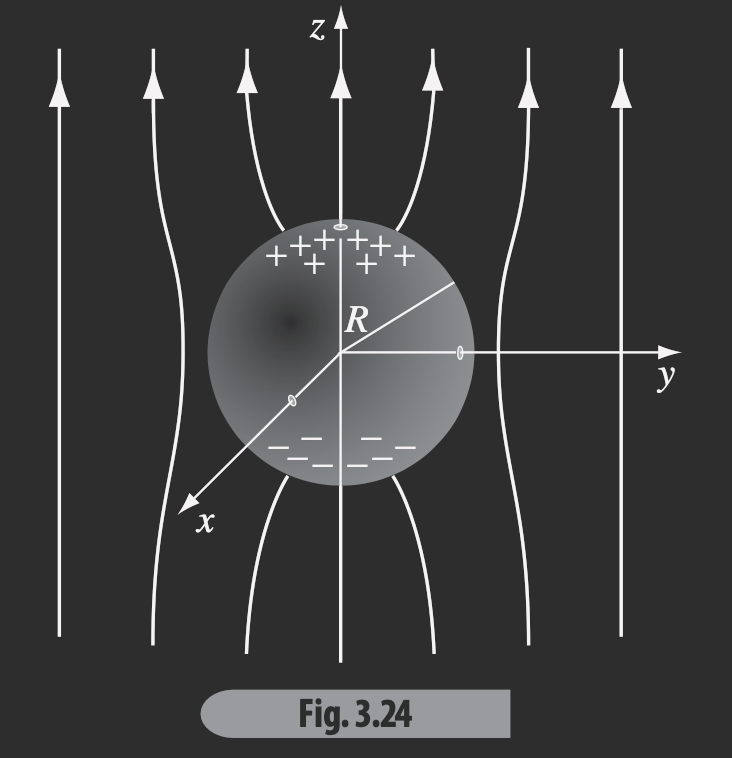
\includegraphics[width=0.4\linewidth]{fig3_24.png}
    \caption{Graph of $V(r,\theta)$}
    \label{fig:lecture3_24}
\end{figure*}

We can see from Fig. \ref{fig:lecture3_24} that the conductor acts as an attractive lens for the field.

Furthermore, the charge distribution on the sphere is
\begin{align*}
    \sigma &= -\epsilon_0 \pdv{V}{n} = \epsilon_0 \pdv{V}{r} \eval_{r = R} \\
    &= 3 \epsilon_0 E_0 \cos\theta
\end{align*}
which is shown in Fig. \ref{fig:lecture3_24b}.
\begin{figure*}[ht]
    \centering
    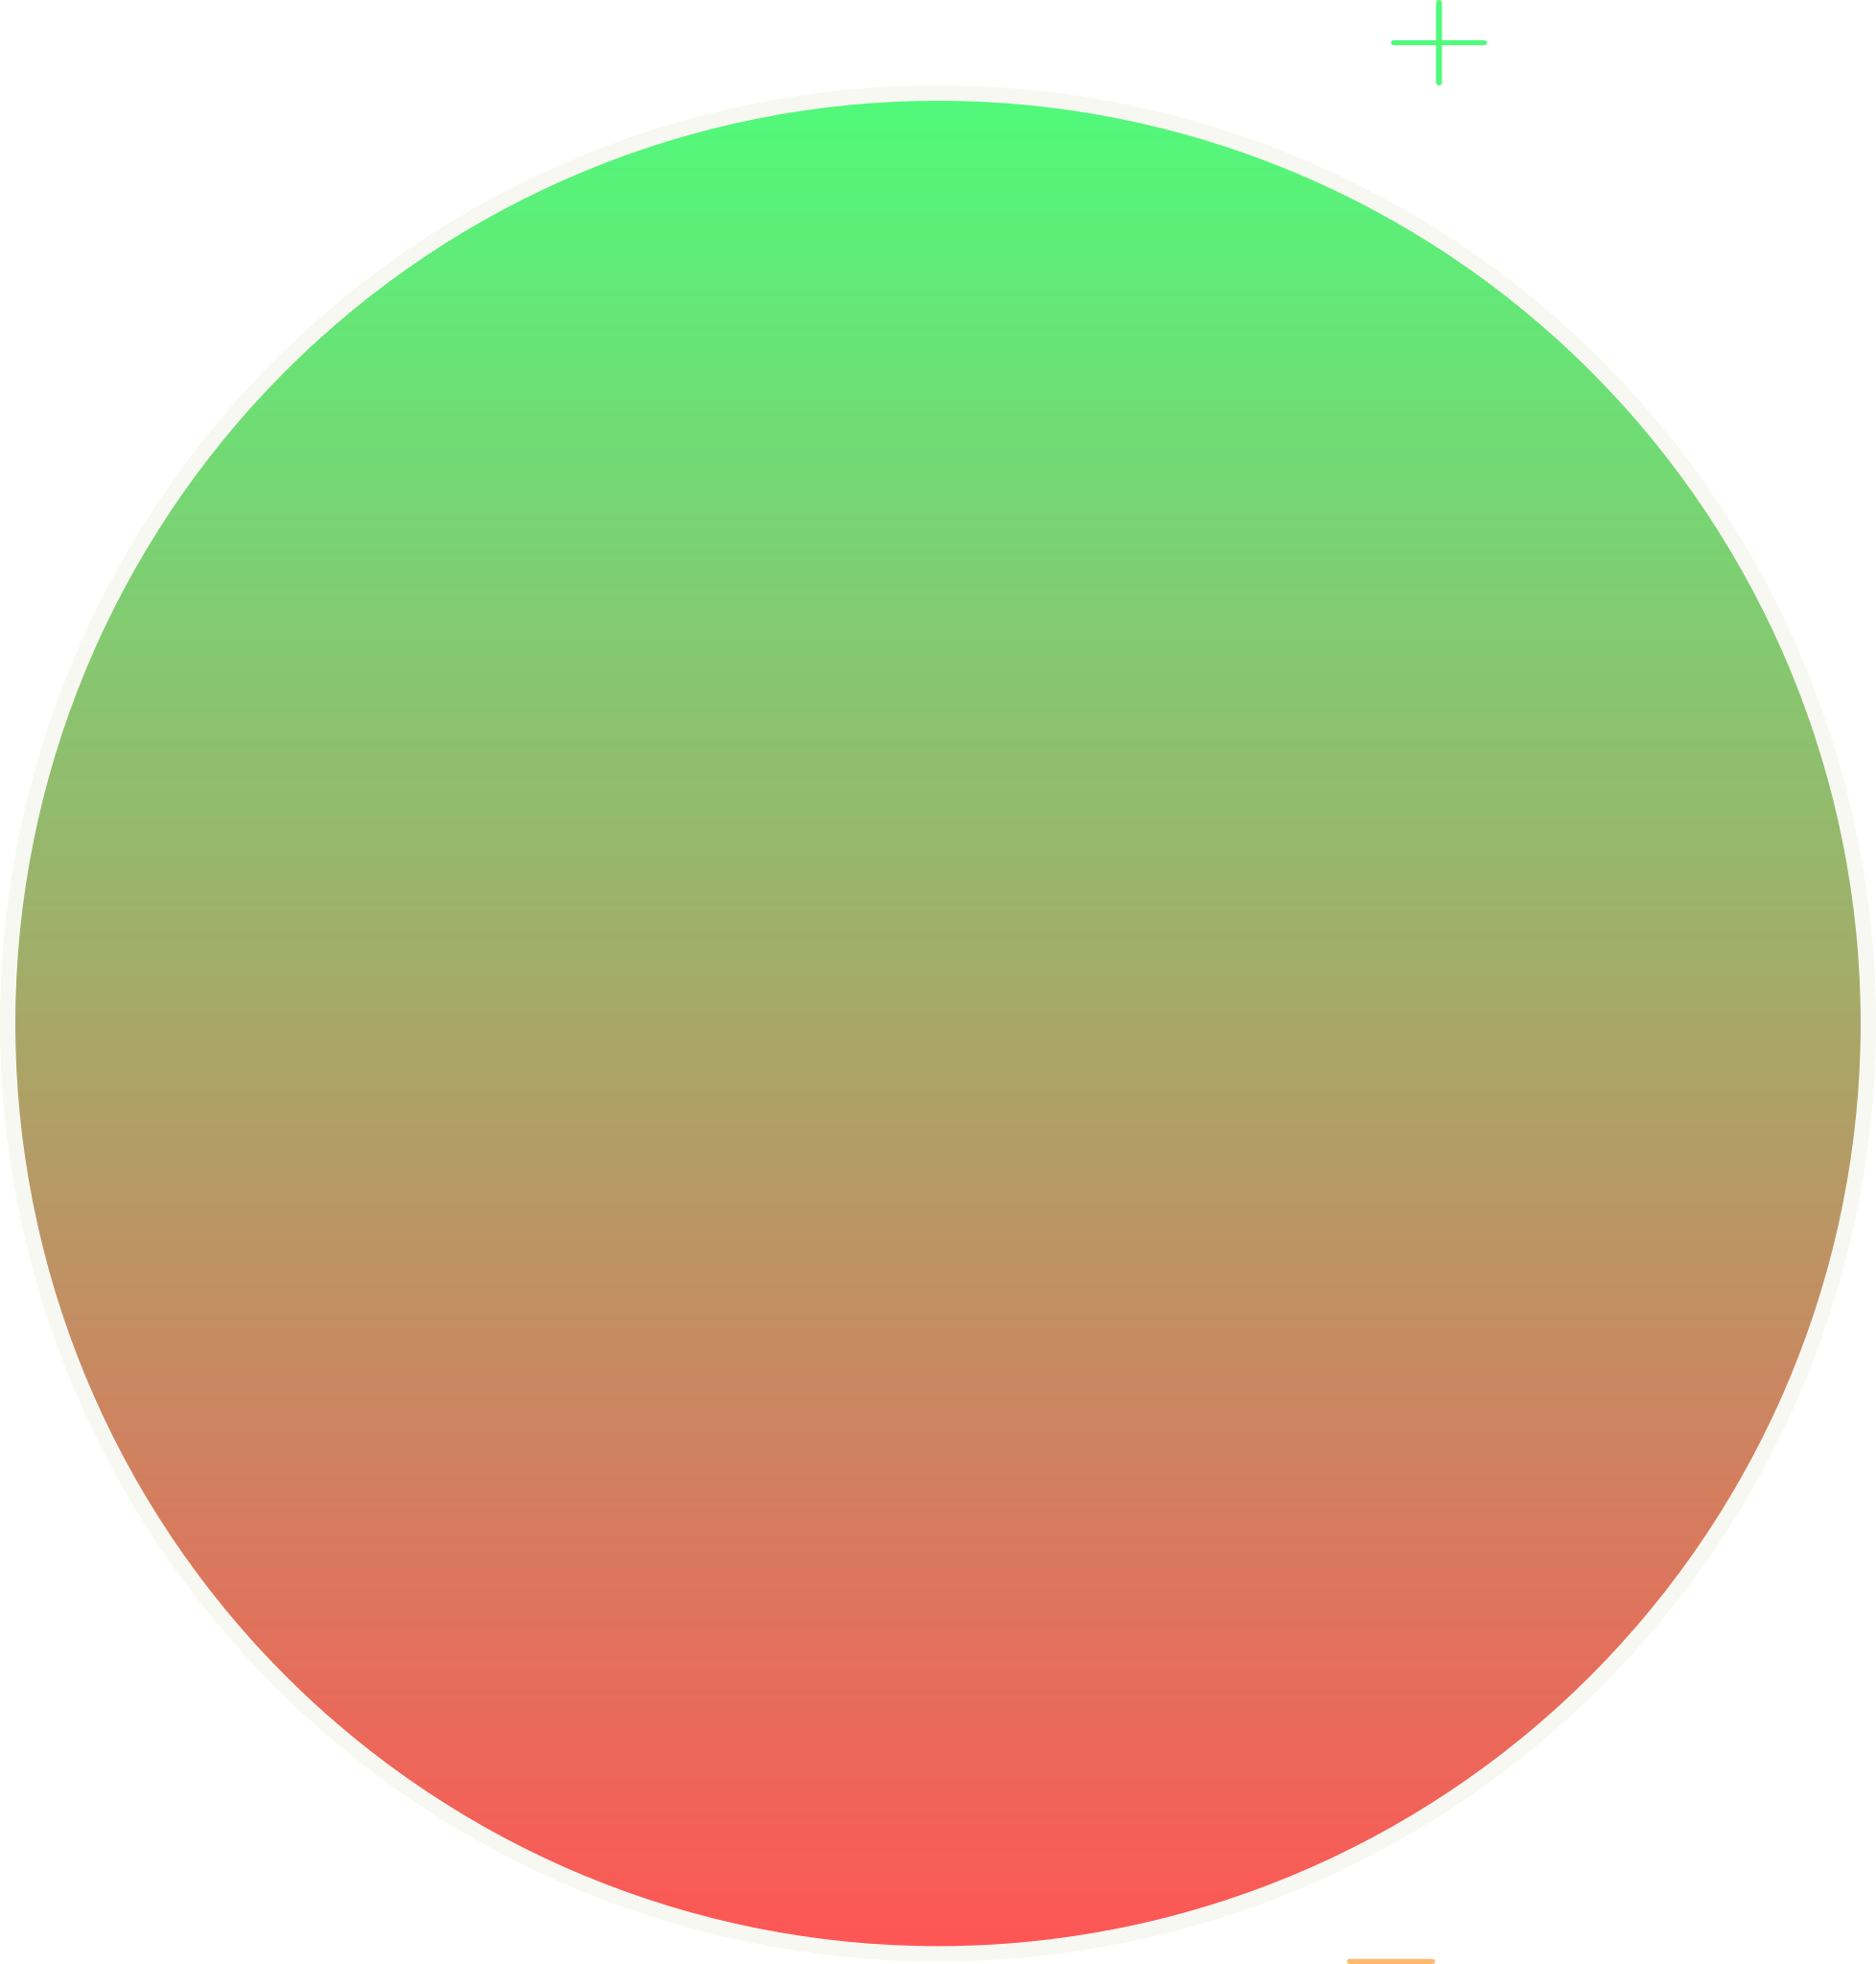
\includegraphics[width=0.4\linewidth]{fig3_24b.png}
    \caption{Charge distribution $\sigma(\theta)$}
    \label{fig:lecture3_24b}
\end{figure*}

\newpage
\subsection{Multipole Expansion}

\subsubsection{To approximate potential at great distances}

\begin{figure*}[ht]
    \centering
    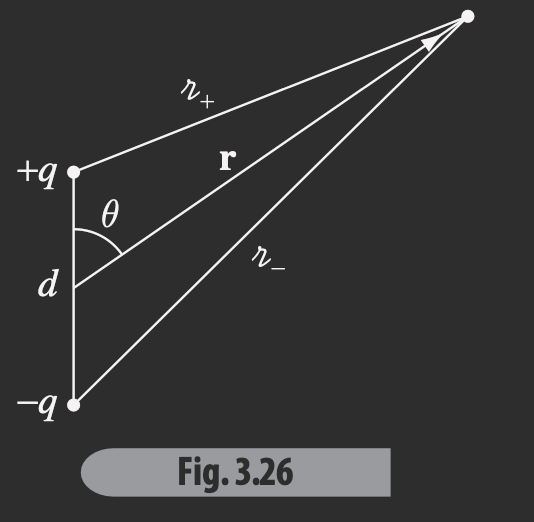
\includegraphics[width=0.4\linewidth]{fig3_26.png}
    \caption{Dipole}
    \label{fig:lec3_26}
\end{figure*}

For a dipole of opposite charge (Fig. \ref{fig:lec3_26}) we are trying to
find the potential $V(\vb r)$ for $r \gg d$. Using superposition
\begin{align*}
    V(\vb r) = \ke \qt(
        \frac{q}{\scriptr_+} - \frac{q}{\scriptr_-}
    )
\end{align*}
And using Law of Cosines
\begin{align*}
    \scriptr_{\pm}^2 &= r^2 + (d/2)^2 \mp rd\cos\theta \\
    &= r^2 \qt(
        1 \mp \frac{d}{r} \cos\theta + \cancel{\frac{d^2}{4r^2}}
    )
\end{align*}
So we solve for $\frac{1}{\scriptr_{\pm}}$ and use binomial expansion:
\begin{align*}
    \frac{1}{\scriptr_{\pm}} = \frac{1}{r} \qt(
        1 \mp \frac{d}{r} \cos\theta 
    )^{-1/2}
    \approx \frac{1}{r} \qt(1 \pm \frac{d}{2r} \cos\theta)
\end{align*}
Thus
\begin{align*}
    V(\vb r) = \ke \frac{qd\cos\theta}{r^2}
\end{align*}

We can abstract this to general multipoles such as the monoponole, quadropole, octopole, hexadecapole, etc. (Fig. \ref{fig:lecture3_27}).

\begin{figure*}
    \centering
    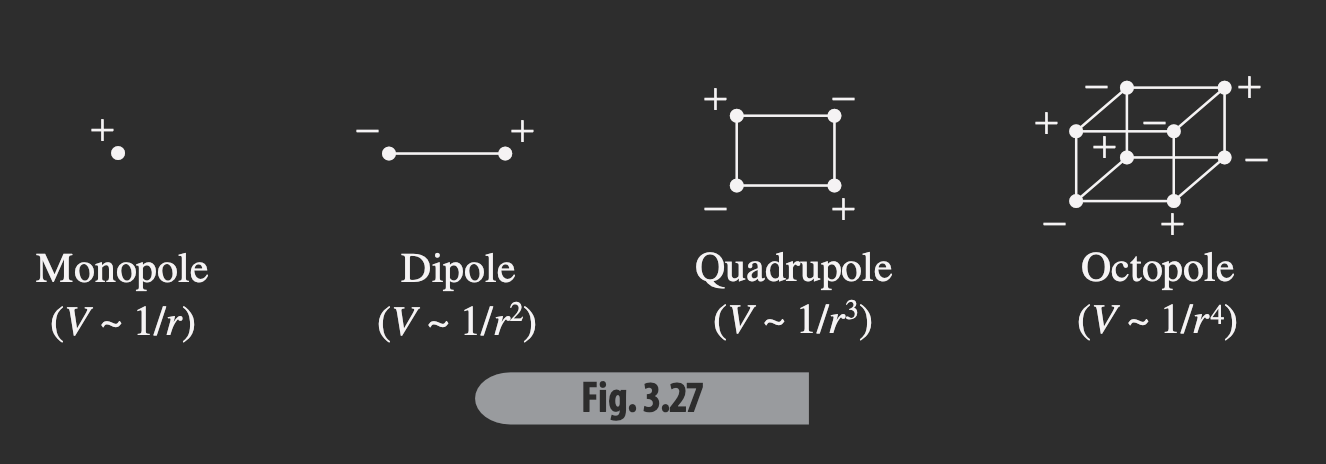
\includegraphics[width=0.4\linewidth]{fig3_27.png}
    \caption{Multipole Expansion}
    \label{fig:lecture3_27}
\end{figure*}

\newpage
Expanding the potential to any local distribution of charge
\begin{figure*}
    \centering
    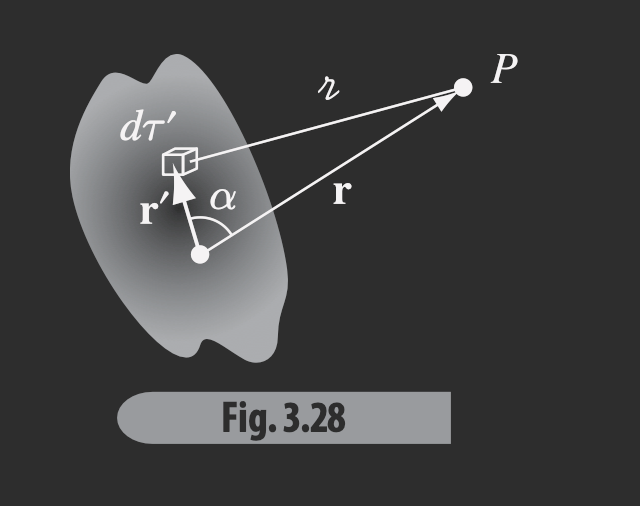
\includegraphics[width=0.4\linewidth]{fig3_28.png}
    \caption{General local charge distribution}
    \label{fig:lecture3_28}
\end{figure*}
Thus
\begin{align*}
    V(\vb r) = \ke \int \frac{\rho(\vb r')}{\scriptr} \dd\tau'
\end{align*}
using LoC again
\begin{align*}
    \scriptr^2 &= r^2 + r'^2 - 2rr'\cos\alpha \\
    &= r^2 \qt[
        1 + \qt(\frac{r'}{r})^2 - 2\frac{r'}{r}\cos\alpha
    ]
\end{align*}
where we let $\scriptr = r\sqrt{1 + \epsilon}$ so
\begin{align*}
    \epsilon = \qt(\frac{r'}{r}) \qt(
        \frac{r'}{r} - 2\cos\alpha
    )
\end{align*}
Far away $\epsilon \ll 1$ so we can binomial expand
\begin{align*}
    \frac{1}{\scriptr} &= \frac{1}{r} (1 + \epsilon)^{-1/2} \\
    &= \frac{1}{r} \qt(
        1 - \frac{\epsilon}{2} + 3/8 \epsilon^2 - \dots
    ) \\
    &= \frac{1}{r} \qt(
        1 - \frac{1}{2} \qt(\frac{r'}{r}) \qt(\frac{r'}{r} - 2\cos\alpha) 
        + \frac{3}{8} \qt(\frac{r'}{r})^2 \qt(\frac{r'}{r} - 2\cos\alpha)^2
        - \frac{5}{16} \qt(\frac{r'}{r})^3 \qt(\frac{r'}{r} - 2\cos\alpha)^3
    ) \\
    &= \frac{1}{r} \qt[
        1 + \frac{r'}{r} \cos\alpha + \qt(\frac{r'}{r})^2 \qt(\frac{3\cos^2\alpha -1}{2})
        + \qt(\frac{r'}{r})^3 \qt(\frac{5\cos^3\alpha - 3\cos\alpha}{2}) + \dots
    ]
\end{align*}
all these terms are related to the Legendre polynomial $P_\ell(\cos\alpha)$ thus we can condense this to
\begin{align*}
    \frac{1}{\scriptr} = \frac{1}{r} \sum_{n = 0}^\infty \qt(\frac{r'}{r})^n P_n (\cos\alpha)
\end{align*}
We can substitute this back into the potential
\begin{align*}
    \boxed{
        V(\vb r) = \ke \sum_{n = 0}^\infty \frac{1}{r^{n+1}} \int (r')^n P_n(\cos\alpha) \rho(\vb r') \dd\tau'
    }
\end{align*}
where each term of the sum is a multipole expansion of $V$ i.e. the monopole ($1/r$), dipole ($1/r^2$), etc.
\newpage
\subsubsection{Monopole \& Dipole}

Obviously the $1/r$ dominates for the monopole i.e.
\begin{align*}
    V_\text{mono} = \ke \frac{Q}{r}
\end{align*}
The dipole is the $n=1$ term
\begin{align*}
    V_\text{dip}(\vb r) = \ke \frac{1}{r^2} \int r' \cos\alpha \rho(\vb r') \dd\tau'
\end{align*}
where $r'\cos\alpha = \vu r \cdot \vb r'$ so
\begin{align*}
    = \ke \frac{1}{r^2} \vu r \cdot \int \vb r' \rho(\vb r') \dd\tau'
\end{align*}
And we define the integral as the dipole moment
\begin{align*}
    \boxed{
        \vb p = \int \vb r' \rho(\vb r') \dd\tau'
    }
\end{align*}
So the dipole potential is simplified to
\begin{align*}
    \boxed{
        V_\text{dip}(\vb r) = \ke \frac{\vb p \cdot \vu r}{r^2}
    }
\end{align*}

For \textit{discrete} charges:
\begin{align*}
    \vb p = \sum_{i=1}^n q_i \vb r_i'
\end{align*}
where for a dipole 
\begin{figure*}[ht]
    \centering
    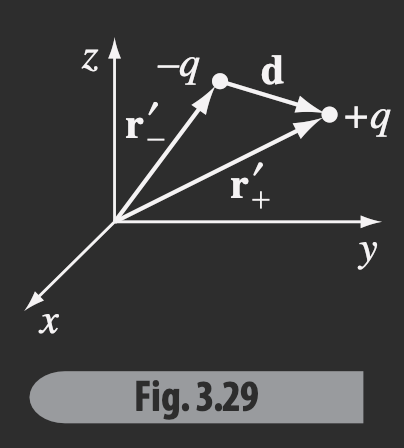
\includegraphics[width=0.3\linewidth]{fig3_29.png}
    \caption{Dipole}
    \label{fig:lecture3_29}
\end{figure*}
\begin{align*}
    \vb p &= q \vb r_+' - q \vb r_-' \\
    &= q(\vb r_+' - \vb r_-') \\
    &= q \vb d
\end{align*}

For a physical or a pure dipole where $\vb d \to 0$ while $q \to \infty$
\begin{align*}
    V_\text{dip} = \ke \frac{\vb p \cdot \vu r}{r^2} = \ke \frac{p \cos\theta}{r^2}
\end{align*}
And looking at the E-field $\vb E = -\grad V$; the components are
\begin{align*}
    E_r &= -\pdv{V}{r} = \ke \frac{2p\cos\theta}{r^3} \\
    E_\theta &= -\frac{1}{r} \pdv{V}{\theta} = \ke \frac{p\sin\theta}{r^3} \\
    E_\phi &= 0
\end{align*}
So
\begin{align*}
    \vb E_\text{dip} = \ke \frac{p}{r^3} \qt(2\cos\theta \vu r + \sin\theta \vu \theta)
\end{align*}
\begin{figure*}[ht]
    \centering
    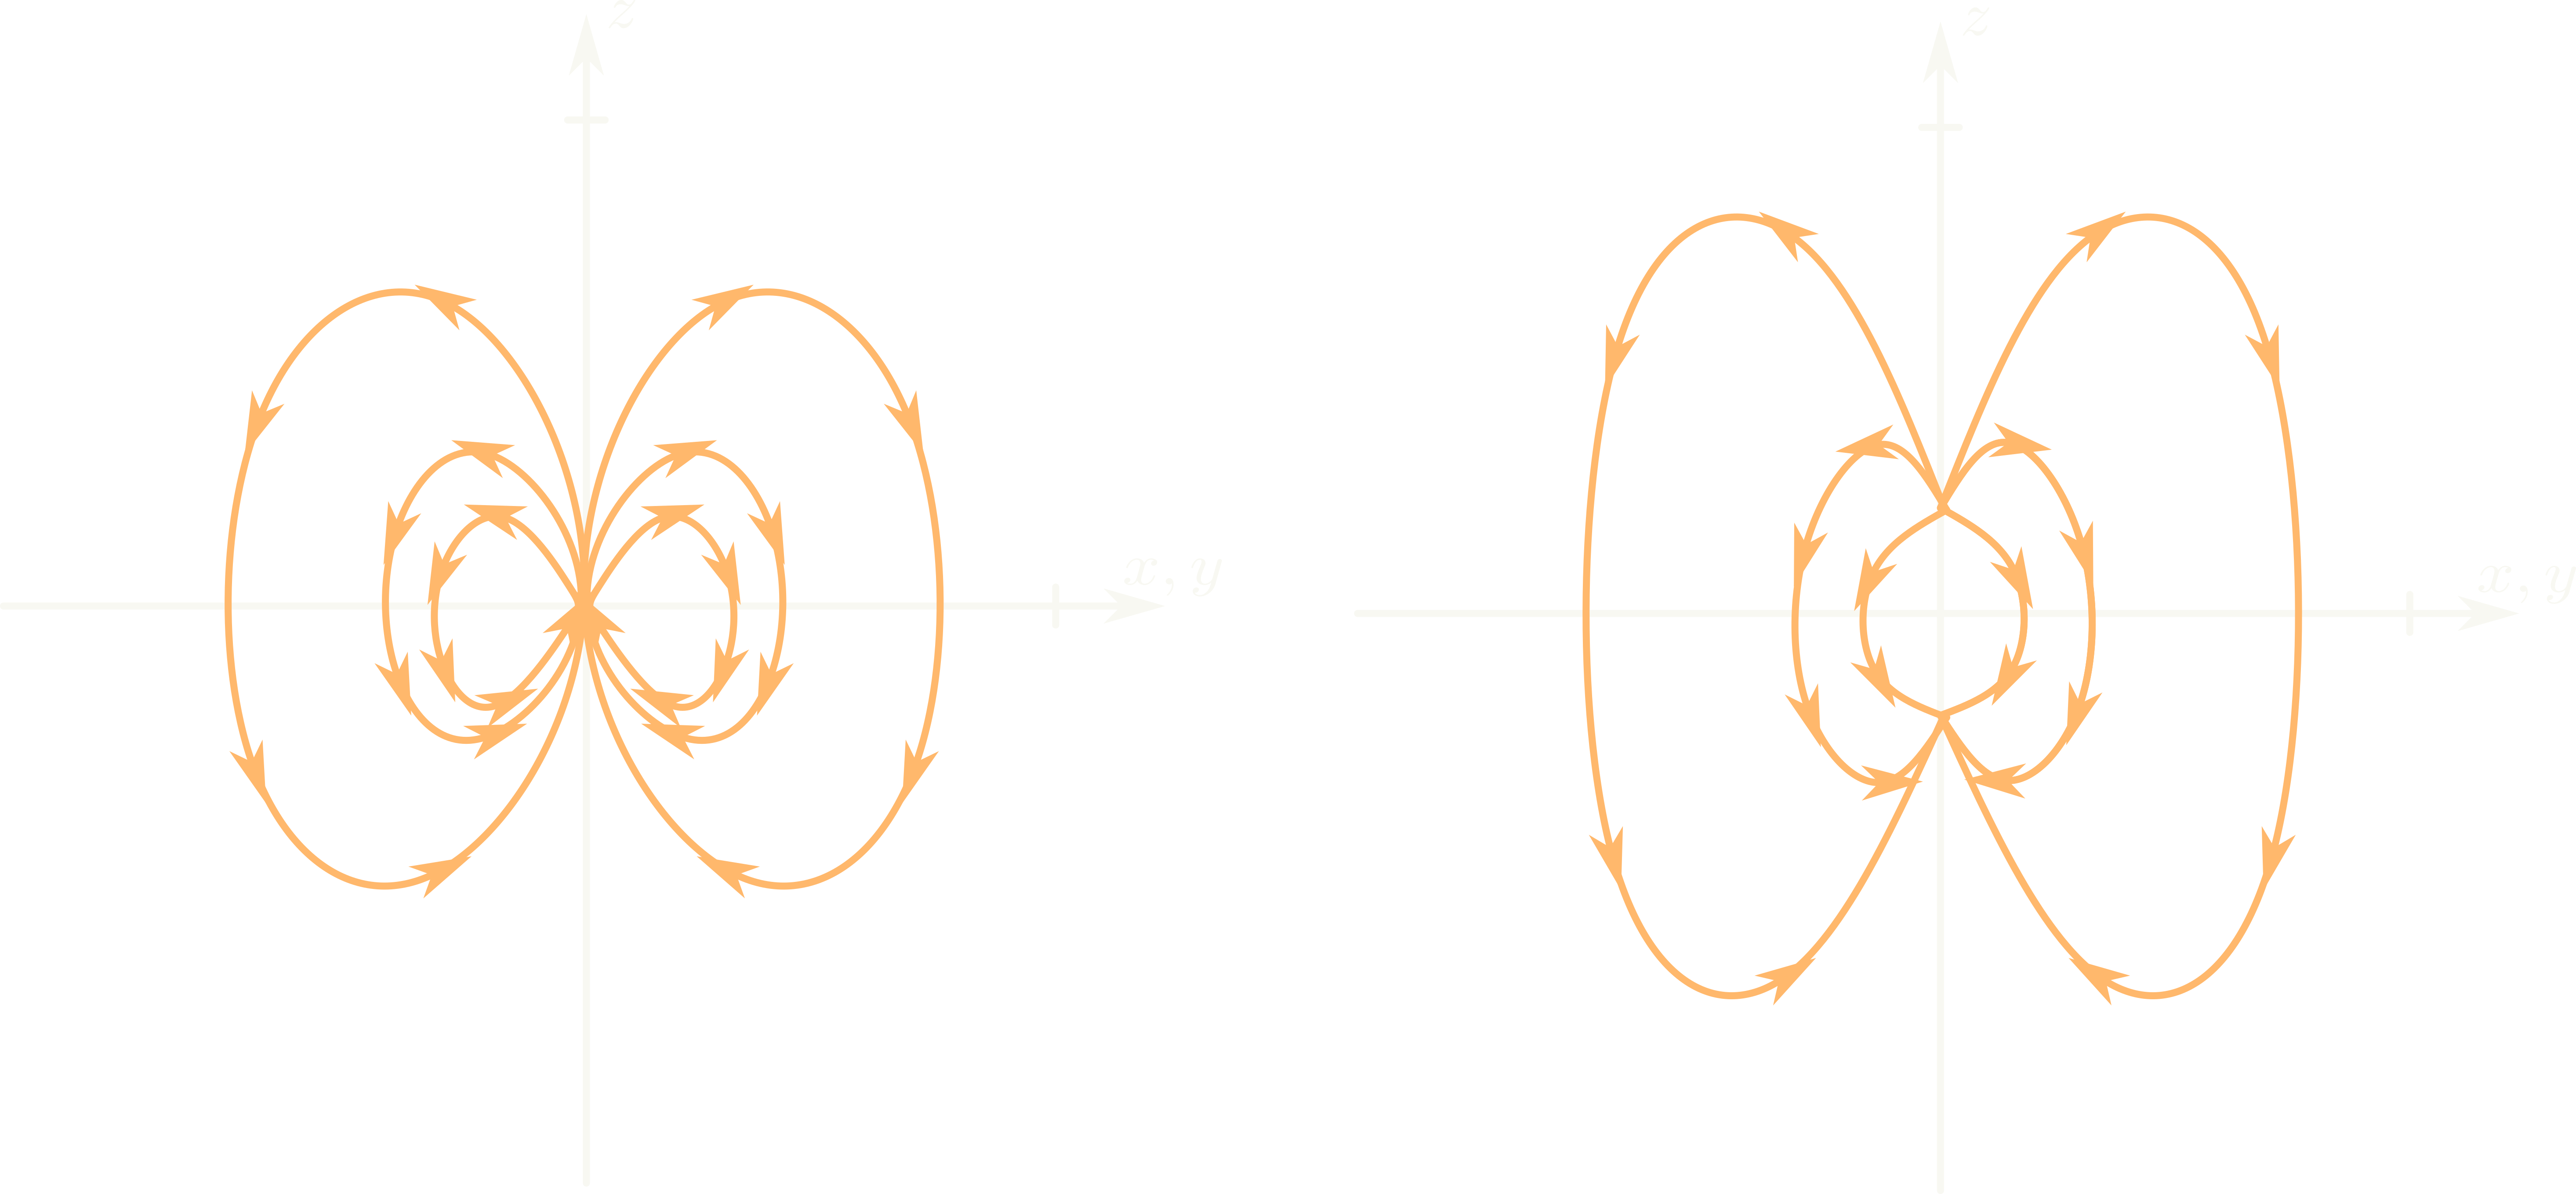
\includegraphics[width=0.5\linewidth]{fig3_29b.png}
    \caption{Pure dipole (left) and physical dipole (right)}
    \label{fig:lecture3_29b}
\end{figure*}
\end{document}